\chapter{Реализация системы составления предварительного расписания} \label{ch3}
В данной главе речь идёт о ПО, рассматривавшемся в качестве средств разработки ситемы составления расписания сессии для СПбПу. В параграфах \ref{ch3:sec1} и \ref{ch3:sec2} приводится обоснование выбора средств реализации системы таких как язык программирования, фреймворков и СУБД. В параграфе \ref{ch3:sec3} приводится архитектура реализованной системы .
	
\section{Выбор языка программирования} \label{ch3:sec1}
Так как система составления расписания сессии должна иметь веб-модуль, необходимо подобрать подходящий для этой цели язык программирования. Среди высокоуровневых языков, которые потенциально могли бы сделать процесс разработки более быстрым, а результат качественным рассматривались следующие претенденты: 
\begin{itemize}
\item  Java;
\item  JavaScript;
\item  C\#;	
\item  C++.	
\end{itemize}

\subsection{Java}
Java - один из самых популярных объектно-ориентированных языков программирования, что всегда является преимуществом, так как количество и качество документации, множество фреймворков и библиотек под любые нужды делает процесс разработки быстрее и эффективнее. Технология Garbage Collection, реализованная в Java оптимизирует управление памятью программ, что очень важно для работы с большим количеством входных данных, как в задаче составления расписания сессии. Также плюсом данного языка является его кроссплатформенность, а значит код на нём может быть запущен везде, где установлена Java Virtual Machine. 

\subsection{JavaScript}
JavaScript - язык программирования, который изначально использовался для разработки фронтенда и с помощью скриптов встраивал в HTML страницы исполняемый код. Сейчас JavaScript можно использовать и в качестве основного языка для написания бэкенда, так как c появлением среды Node.js программы на JavaScript можно запускать и на сервере. Преимуществом JavaScript всё ещё является его ориентированность на работу с веб страницами, а также его простота. Скрипты на этом языке поддерживаются всеми современными браузерами и не требуют установки дополнительного программного обеспечения. В качестве языка для бэкенда недостатком служит отсутствие явной типизации, а так же разработку усложняет тот факт, что нет возможности узнать об ошибке на этапе компиляции, а значит о том, что где-то в коде появилось сложение строки с счислом, разработчик узнает только тогда, когда программа выполнится до этого места и не раньше. 

\subsection{C\#}
C\#, как и Java, является кроссплатформенным языком программирования, который разработан для создания приложений среды NET Framework. С точки зрения разработки C\# удобен обилием синтаксического сахара, за счёт которого упраздняются громоздкие конструкции, делающие написание кода более бастрым, а также повышающие его читаемость. Это в какой-то мере сказывается на производительности вычислений, но окупается удобством разработки. Помимо этого для C\# тоже существует множество фреймворков, что также предоставляет возможность переиспользовать уже готовые технологии.

\subsection{C++}
C++ - объектно-ориентированный язык программирования с возможностью низкоуровневой работы с данными, что даёт возможность писать на нём даже микроконтроллеры. Но сложность синтаксиса и небогатая стандартная библиотека затрудняет высокоуровневую разработку. C++ достаточно популярен и имеет большое количество документации, но даже с ней не всегда легко правильно самостоятельно обеспечить грамотную работу с памятью. Ещё одним недостатком этого языка является зависимость от платформы и этот фактор перевешивает даже отличную производительность этого языка.

\subsection{Определение языка программирования}
Для реализации сервиса составления предварительного расписания сессии к языку программирования предъявлялись следующие требования:
\begin{itemize}
\item Наличие подробной документации;
\item Наличие фреймворков для упрощения работы с базой данных и веб-сервисом программы;
\item Кроссплатформенность;
\item Удобство и скорость разработки.
\end{itemize}

Язык Java удовлетворяет всем перечисленным критериям благодаря своей популярности среди программистов. Это существенно упрощает процесс разработки, так как для Java существует множество пособий, а способы устранения возникающих ошибок уже в большинстве собой описаны на различных интернет-ресурсах. Далее выбор фреймворков будет рассматриваться именно для Java, благо для данного языка их существует достаточно. Но стоит заметить, что язык JavaScript, хоть и не очень хорошо подходит для основоного языка в этом проекте, но будет использоваться для создания веб-интерфейса, так как Java не очень хорошо приспособлена для этой задачи.

\section{Выбор фреймворка для построения веб-приложения} \label{ch3:sec2}
\subsection{Spring}
Spring - Java-фреймворк, состоящий из множества компонентов таких как Inversion of Control для управления объектами, MVC для расширения Servlet API и прозрачного разделения между слоями модель, представление, контроллер и даже компонента доступа к базам данных \cite{spring}. Все эти и другие компоненты могут добавляться в проект независимо, что делает разработку более гибкой. Наличие этих модулей избавляет разработчика от низкоуровневой работы с запросами, налаживания взаимодействия с базами данных и прочих моментов имеющих чисто технический характер и не имеющих связи с бизнес-задачей программы. Ещё одним преимуществом Spring  для разработчика является его популярность и качественная документация, чего часто не хватает молодым и мало известным проектам.

\subsection{Dropwizard}
Dropwizard - это фреймворк для создания веб-сервисов RESTful \cite{dropwizard}. Он по умолчанию поставляется с такими библиотеками, как Jetty server, Jackson, Metrics, Hibernate Validator и Guava. Dropwizard не имеет русскоязычной документации, что является недостатком. Так же у Dropwizard не так много модулей, как у Spring, но всё ещё просто расширяется с использованием файлов конфигураций.

\subsection{Vert.x}
Vert.x - это асинхронный, событийно ориентированный фреймворк, создатели которого во многом вдохновлялись фреймворком node.js \cite{vertx}. Он позволяет оптимизировать параллельную отправку и получение запросов, обрабатывая их большее количество с меньшими ресурсами, нежели фреймворки, основанные на блокирующем асинхронном вводе-выводе. Vert.x позволяет работать с действительно нагруженными системами, но не имеет такого же количества модулей для разных целей, как Dropwizard и тем более Spring.

\subsection{Определение фреймворка для построения веб-приложения} 
Для написания системы составления расписания сессии СПбПу из рассмотренных фреймворков был выбран именно Spring, потому что обладает всеми необходимыми для данной задачи модулями. Огромное количество библиотек, включённых в Spring может помочь при дальнейшем расширении сервиса без переписывания его на другой фреймворк. Также при поддержании работы системы другими разработчиками не возникнет проблемы с изучением Spring, потому что для него существует множество справочных материалов в том числе на русском языке.

\subsection{Хранение данных}
Spring Framework имеет поддержку ORM Hibernate \cite{hibernate}. ORM или Object-Relational Mapping - это технология, позволяющая сопоставлять объекты объекно-ориентрованной модели, на которой зиждится Java, с сущностями базы данных. Таким образом, не нужно вручную создавать таблицы с полями, соответствующими структуре Java - объекта, ведь можно просто добавить к нему аннотацию, а Hibernate сделает всё автоматически, а самое главное автоматически преобразует полученные результаты select-запроса в объект, что не всегда просто делать самостоятельно. Также, Hibernate имеет предопределённые запросы к базе данных, из-за чего можно не прописывать монотонные sql-запросы на поиск и удаления элемента по id или добавления его в таблицу.

Hibernate поддерживает диалекты и MySQL, и Oracle, и Microsoft SQL Server, и PostgreSQL, поэтому в качестве СУБД была выбрана PostgreSQL, так как она полностью бесплатна и проста в установке на любой платформе.

\subsection{Выводы}
Таким образом, в качестве основного языка программирования был выбран Java, который во фронтенд части дополняется JavaScript, более приспособленным для реализации интерфейсов. Среди фреймворков для работы с веб-приложениями для Java выбор пал на Spring Framework, имеющий множество разным модулей, в том числе Hibernate, с помощью которого осуществляется взаимодействие с базой данной PostgreSQL.

\section{Архитектура системы} \label{ch3:sec3}
На схеме \ref{fig:arch} представлена архитектура система составления предварительного расписания сессии СПбПУ.

\begin{minipage}{\textwidth}
	\centering
	\vspace{\mfloatsep} % интервал  	
	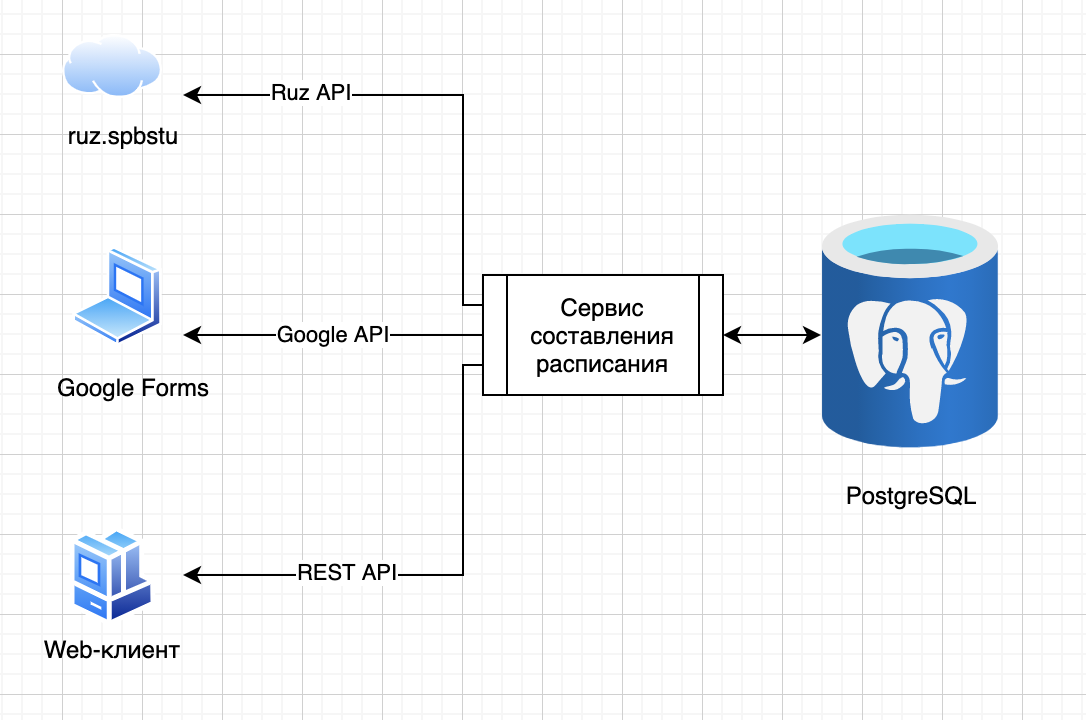
\includegraphics[ keepaspectratio=true, scale=0.6] {my_folder/images/arch}
	\captionof{figure}{Схема архитектуры системы}\label{fig:arch}  
	\vspace{\mfloatsep} % интервал  	
\end{minipage}

Администратор имеет доступ к веб-интерфейсу приложения. С его помощью сведения о том, для каких аттестаций, групп, на какие даты и время должно быть составлено расписание. Spring сервер сохраняет эти данные в базе данных. Полученные сведения дополняются информацией с сайта расписания университета по API. На основе имеющихся данных сервер с помощью Google API формирует форму для сбора сведений преподавательского состава. 
После получения с помощью Google API информации о пожеланиях преподавателей на сервере происходит генерация предварительного расписания и выгрузка его в google-таблицу.

Далее рассмотрим каждое из данных звеньев системы подробнее.

\subsection{Веб-клиент и UI}
 Веб-клиент позволяет администратору работать с системой составления расписания. "Общение" пользователя с сервером осуществляется с помощью REST-запросов на сервер, написанных на JavaScript. Этот код представлен в приложении \ref{appendix-js}
 
 \begin{minipage}{\textwidth}
 	\centering
 	\vspace{\mfloatsep} % интервал  	
 	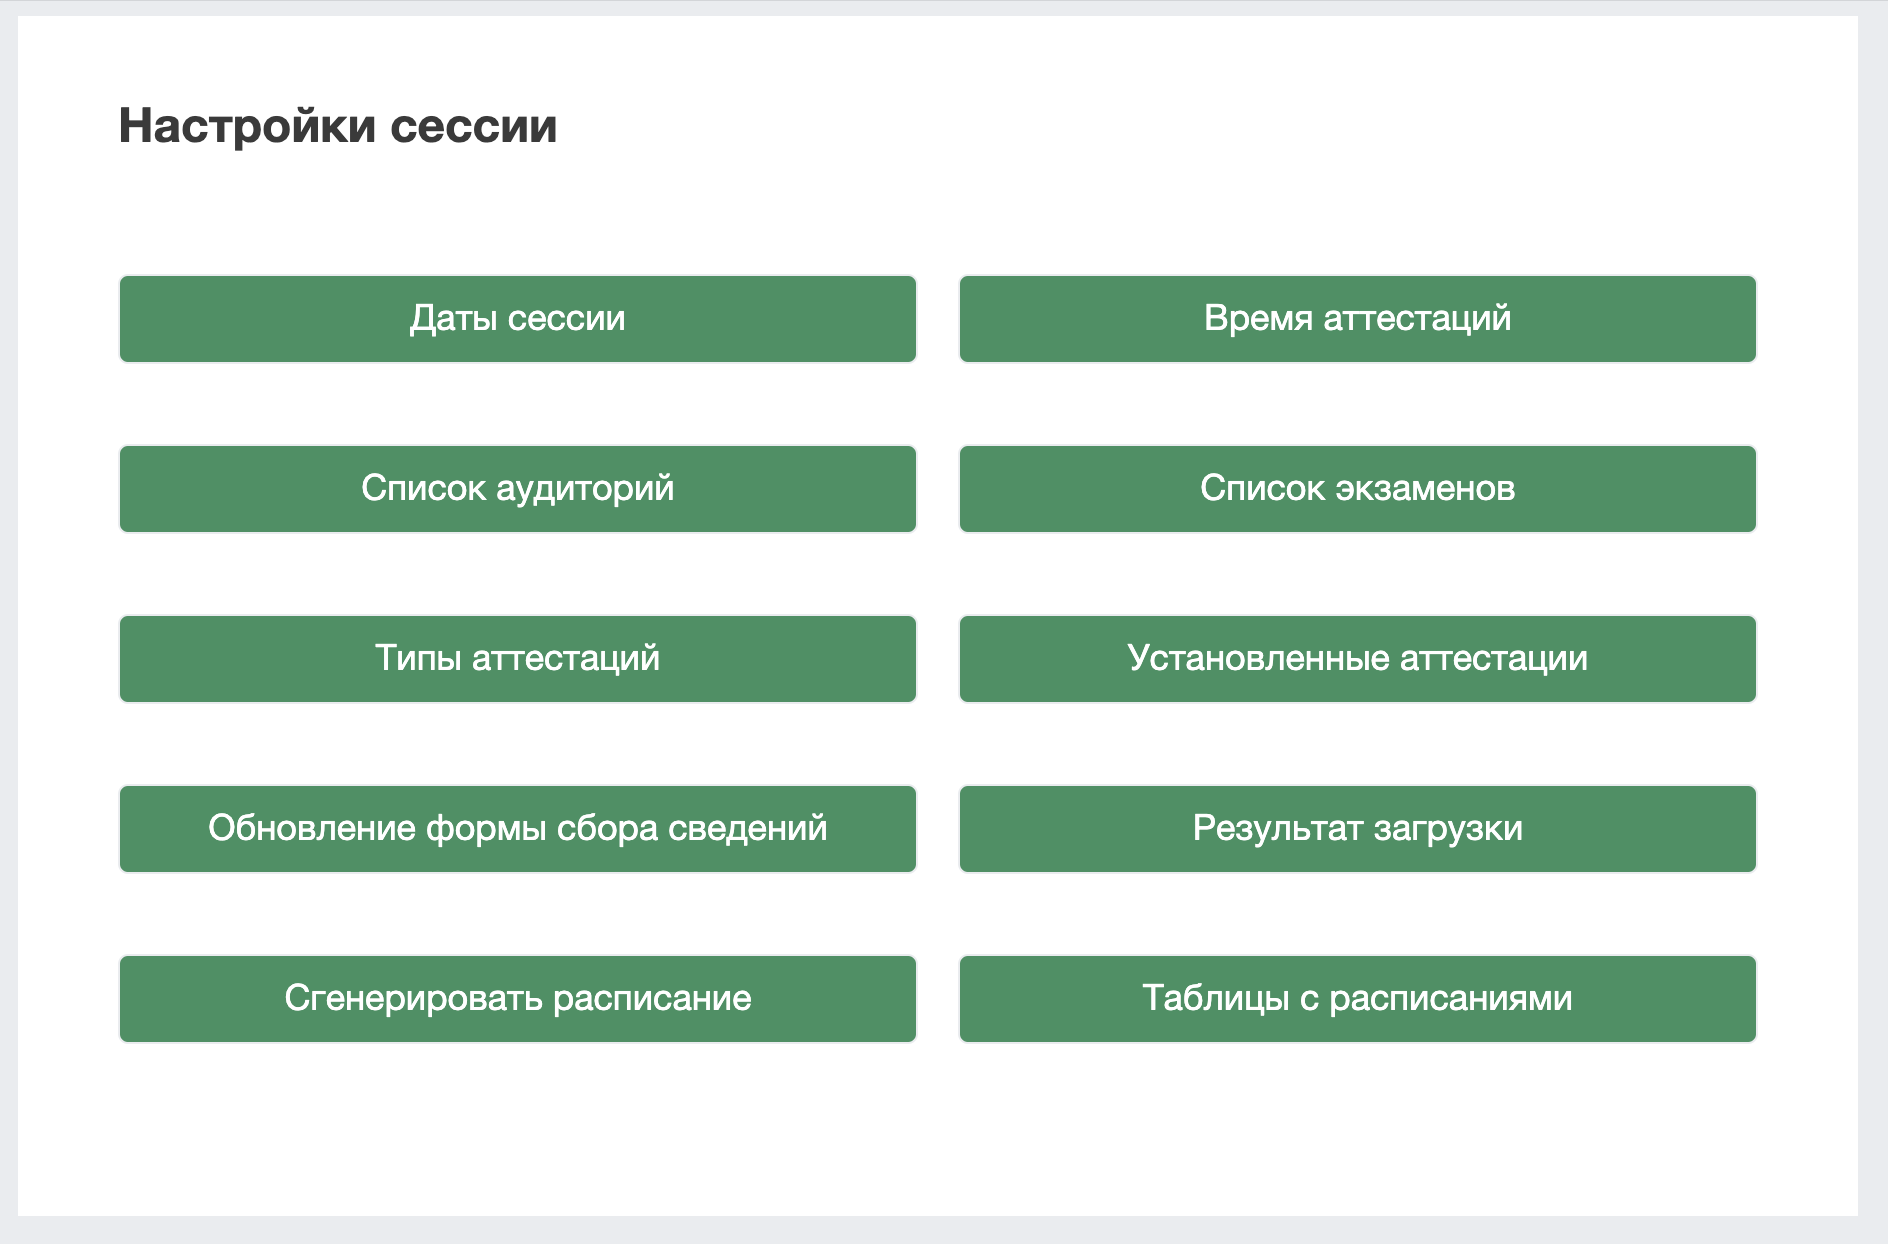
\includegraphics[ keepaspectratio=true, scale=0.4] {my_folder/images/index}
 	\captionof{figure}{Главная страница интерфейса администратора}\label{fig:index}  
 	\vspace{\mfloatsep} % интервал  	
 \end{minipage}

 На рисунке \ref{fig:index} представлен перечень действий, который может выполнить администратор.
 Они реализуются рядом POST-запросов.

POST-запрос к /session/update\_date c параметром days позволяет выбрать дни сессии. Форма для выбора дат изображена на скриншоте \ref{fig:dates}.

\begin{minipage}{\textwidth}
	\centering
	\vspace{\mfloatsep} % интервал  	
	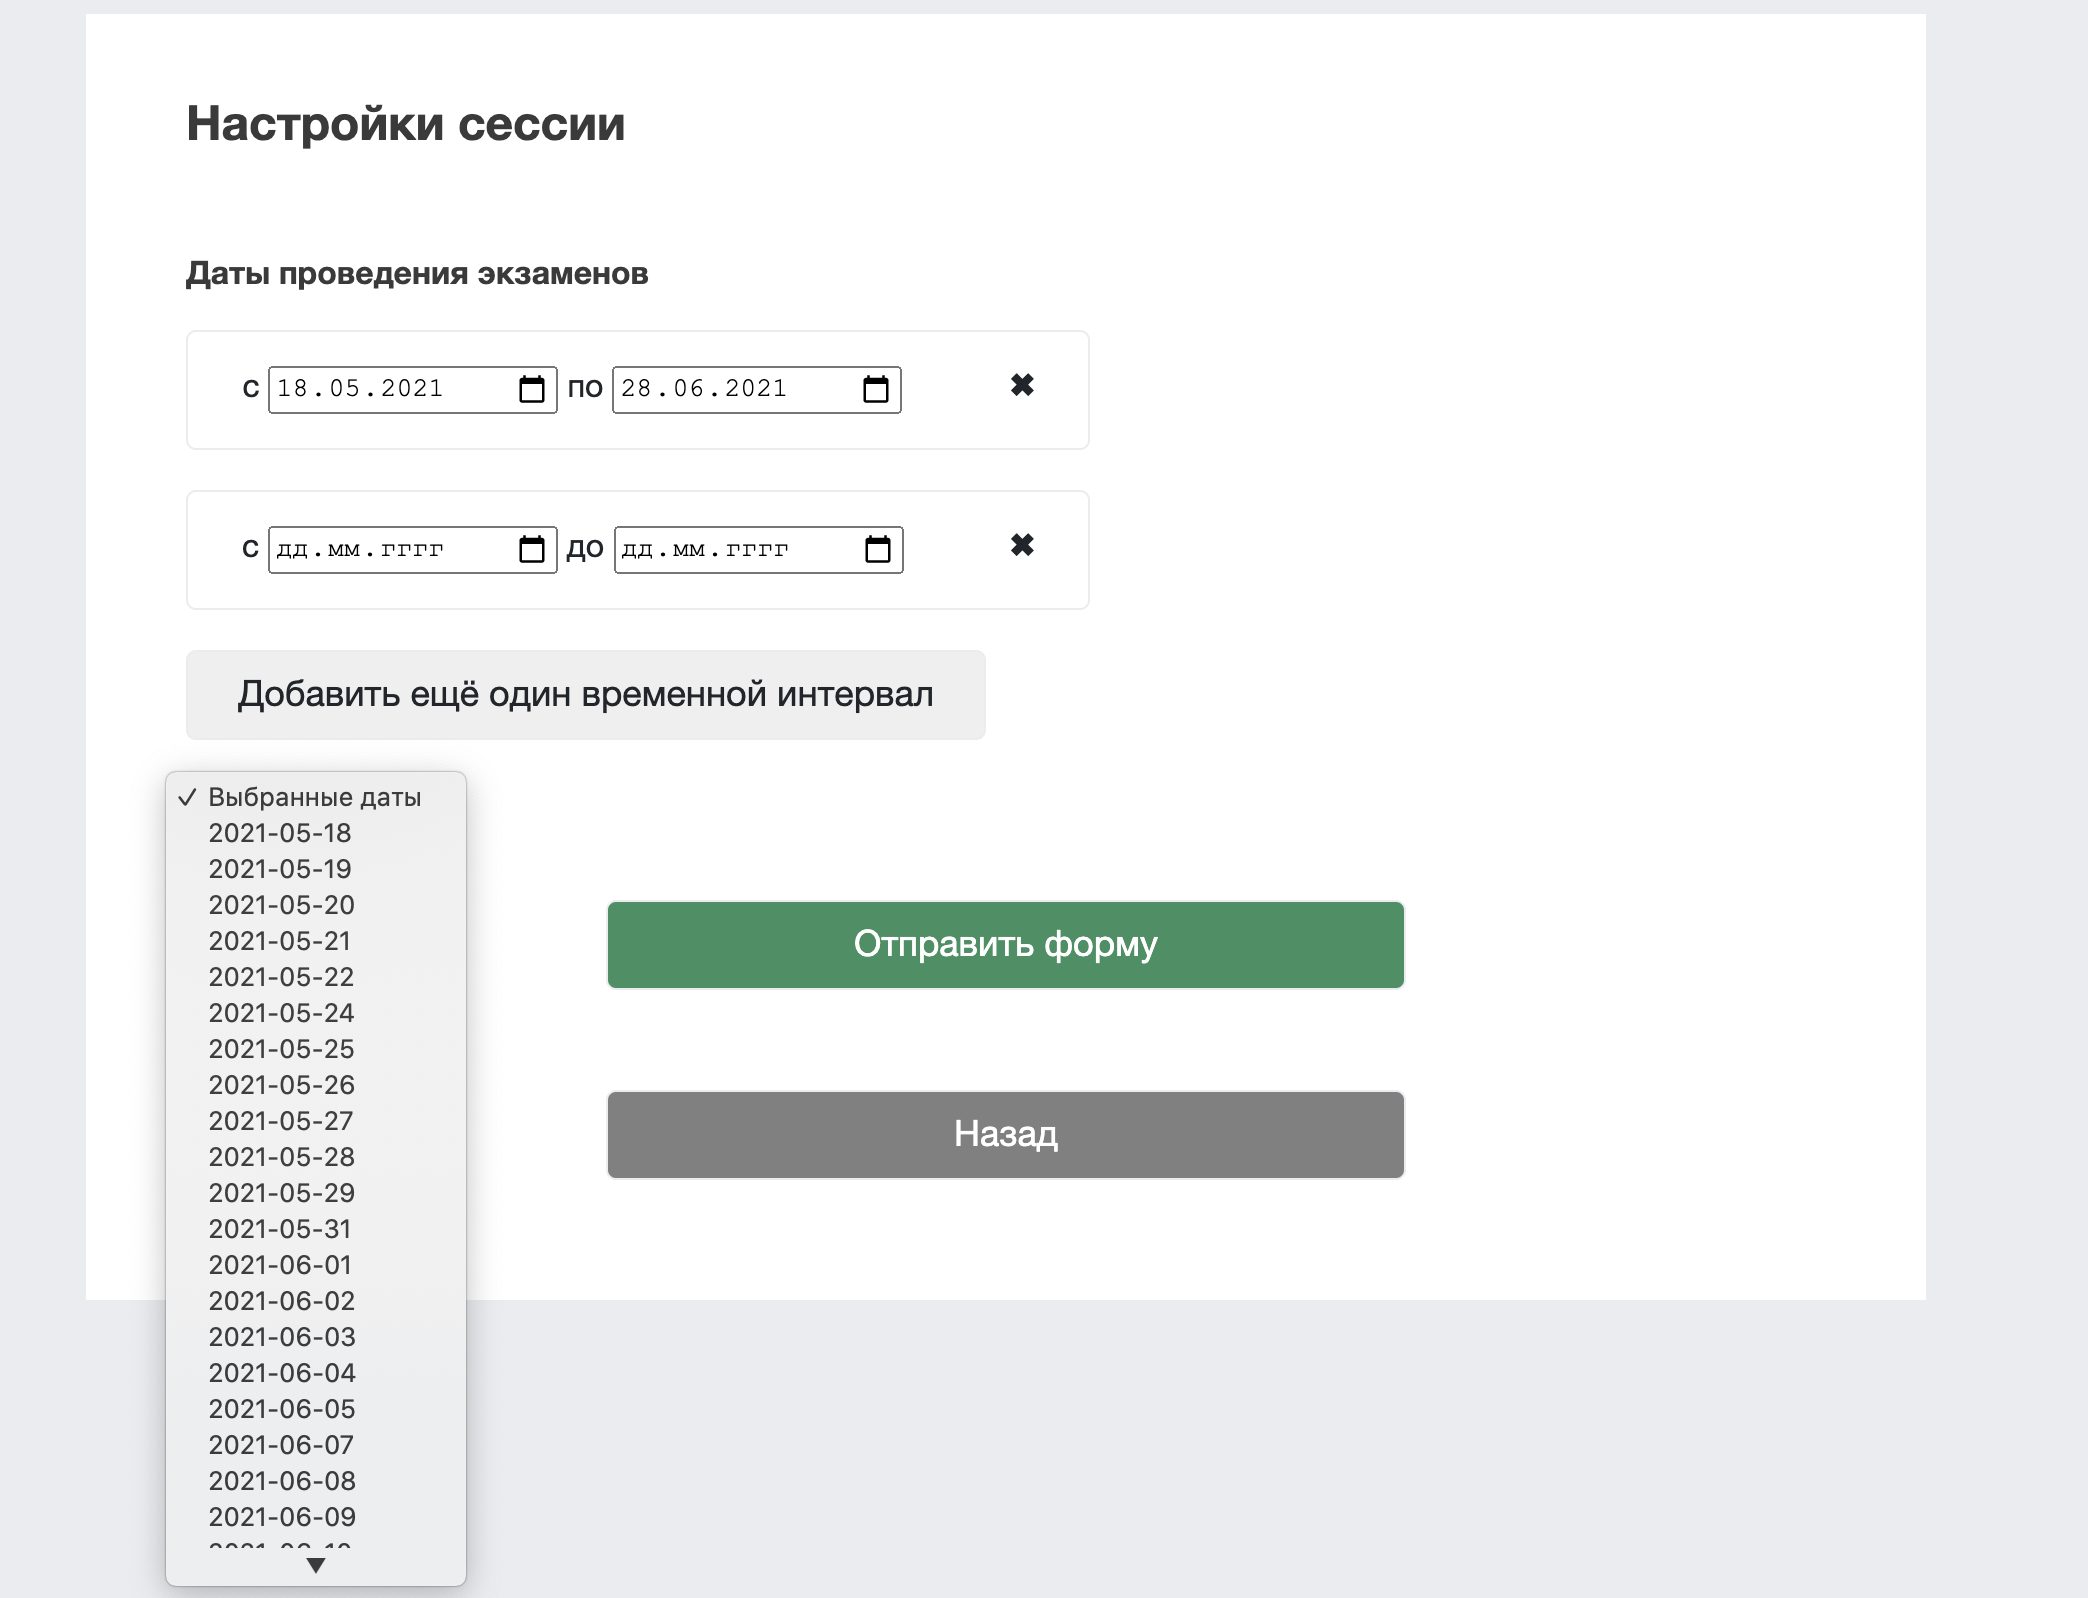
\includegraphics[ keepaspectratio=true, scale=0.4] {my_folder/images/dates}
	\captionof{figure}{Форма выбора дней}\label{fig:dates}  
	\vspace{\mfloatsep} % интервал  	
\end{minipage}
\FloatBarrier

POST-запрос к /session/update\_class c параметром classroomFile позволяет добавить файл с данными об аудиториях, а запрос к  /session/update\_att c параметром attestationFile позволяет загрузить файл с данными о типах аттестаций.

POST-запрос к /session/update\_time c параметрами time1 и time2 позволяет выбрать время проведения аттестаций. Форма для выбора времени изображена на скриншоте \ref{fig:time}.

\begin{minipage}{\textwidth}
	\centering
	\vspace{\mfloatsep} % интервал  	
	
\includegraphics[ keepaspectratio=true, scale=0.5] {my_folder/images/time}
	\captionof{figure}{Форма выбора времени}\label{fig:time}  
	\vspace{\mfloatsep} % интервал  	
\end{minipage}
\FloatBarrier

POST-запросы к /session/update\_exam\_teacher и /session/update\_exam c параметрами spec и examFile позволяет для конкретных специальностей загружать файлы со списком экзаменов. Форма для загрузки учебных планов представлена на скриншоте \ref{fig:plans}.

\begin{minipage}{\textwidth}
	\centering
	\vspace{\mfloatsep} % интервал  	
	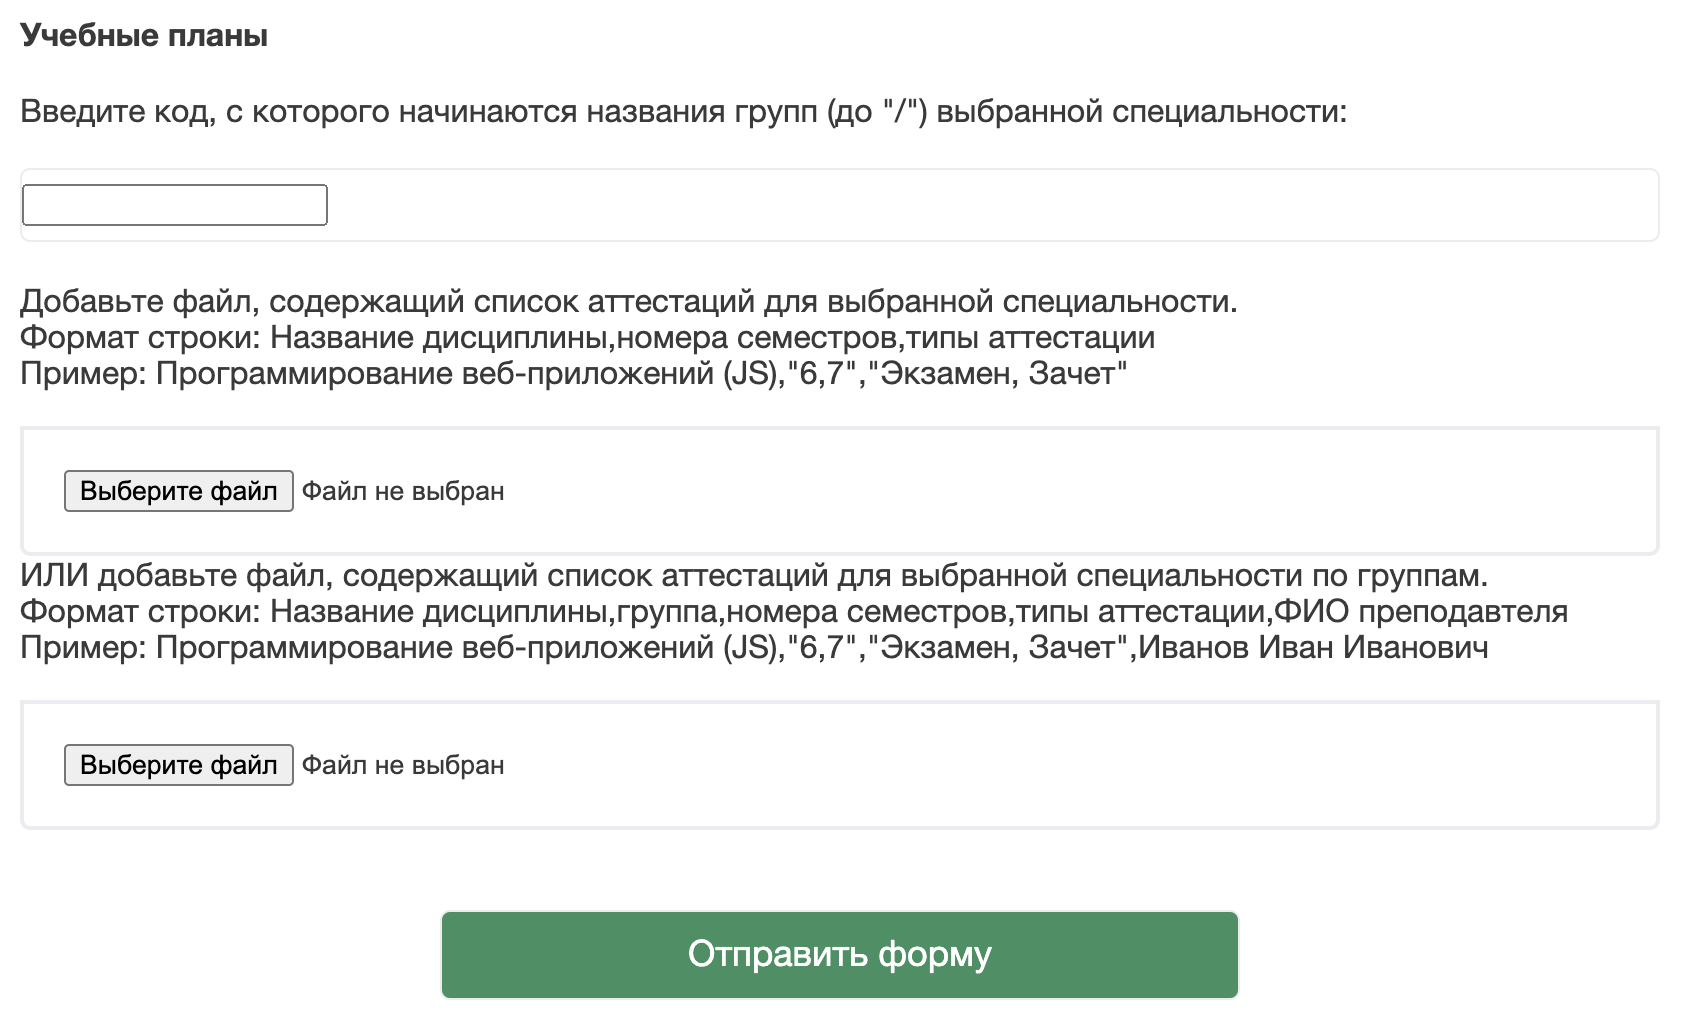
\includegraphics[ keepaspectratio=true, scale=0.5] {my_folder/images/plans}
	\captionof{figure}{Форма загрузки учебных планов}\label{fig:plans}  
	\vspace{\mfloatsep} % интервал  	
\end{minipage}
\FloatBarrier

POST-запрос к /session/update\_external c параметром externalId позволяет добавить идентификатор google-таблицы, в которой содержатся аттестации с известными датами, временем и аудиториями, а запрос к /session/teachers/update c параметром spec даёт возможность обновить google-таблицу с данными для формирования google-формы сбора предпочтений ППС к расписанию сессии.

С помощью POST-запроса к /session/result/create c параметрами spec и levels для выбранных специальностей и курсов генерируется предварительное расписание. Страница с выбором специальностей и курсов для создания расписания представлена на рисунке \ref{fig:generate}.

\begin{minipage}{\textwidth}
	\centering
	\vspace{\mfloatsep} % интервал  	
	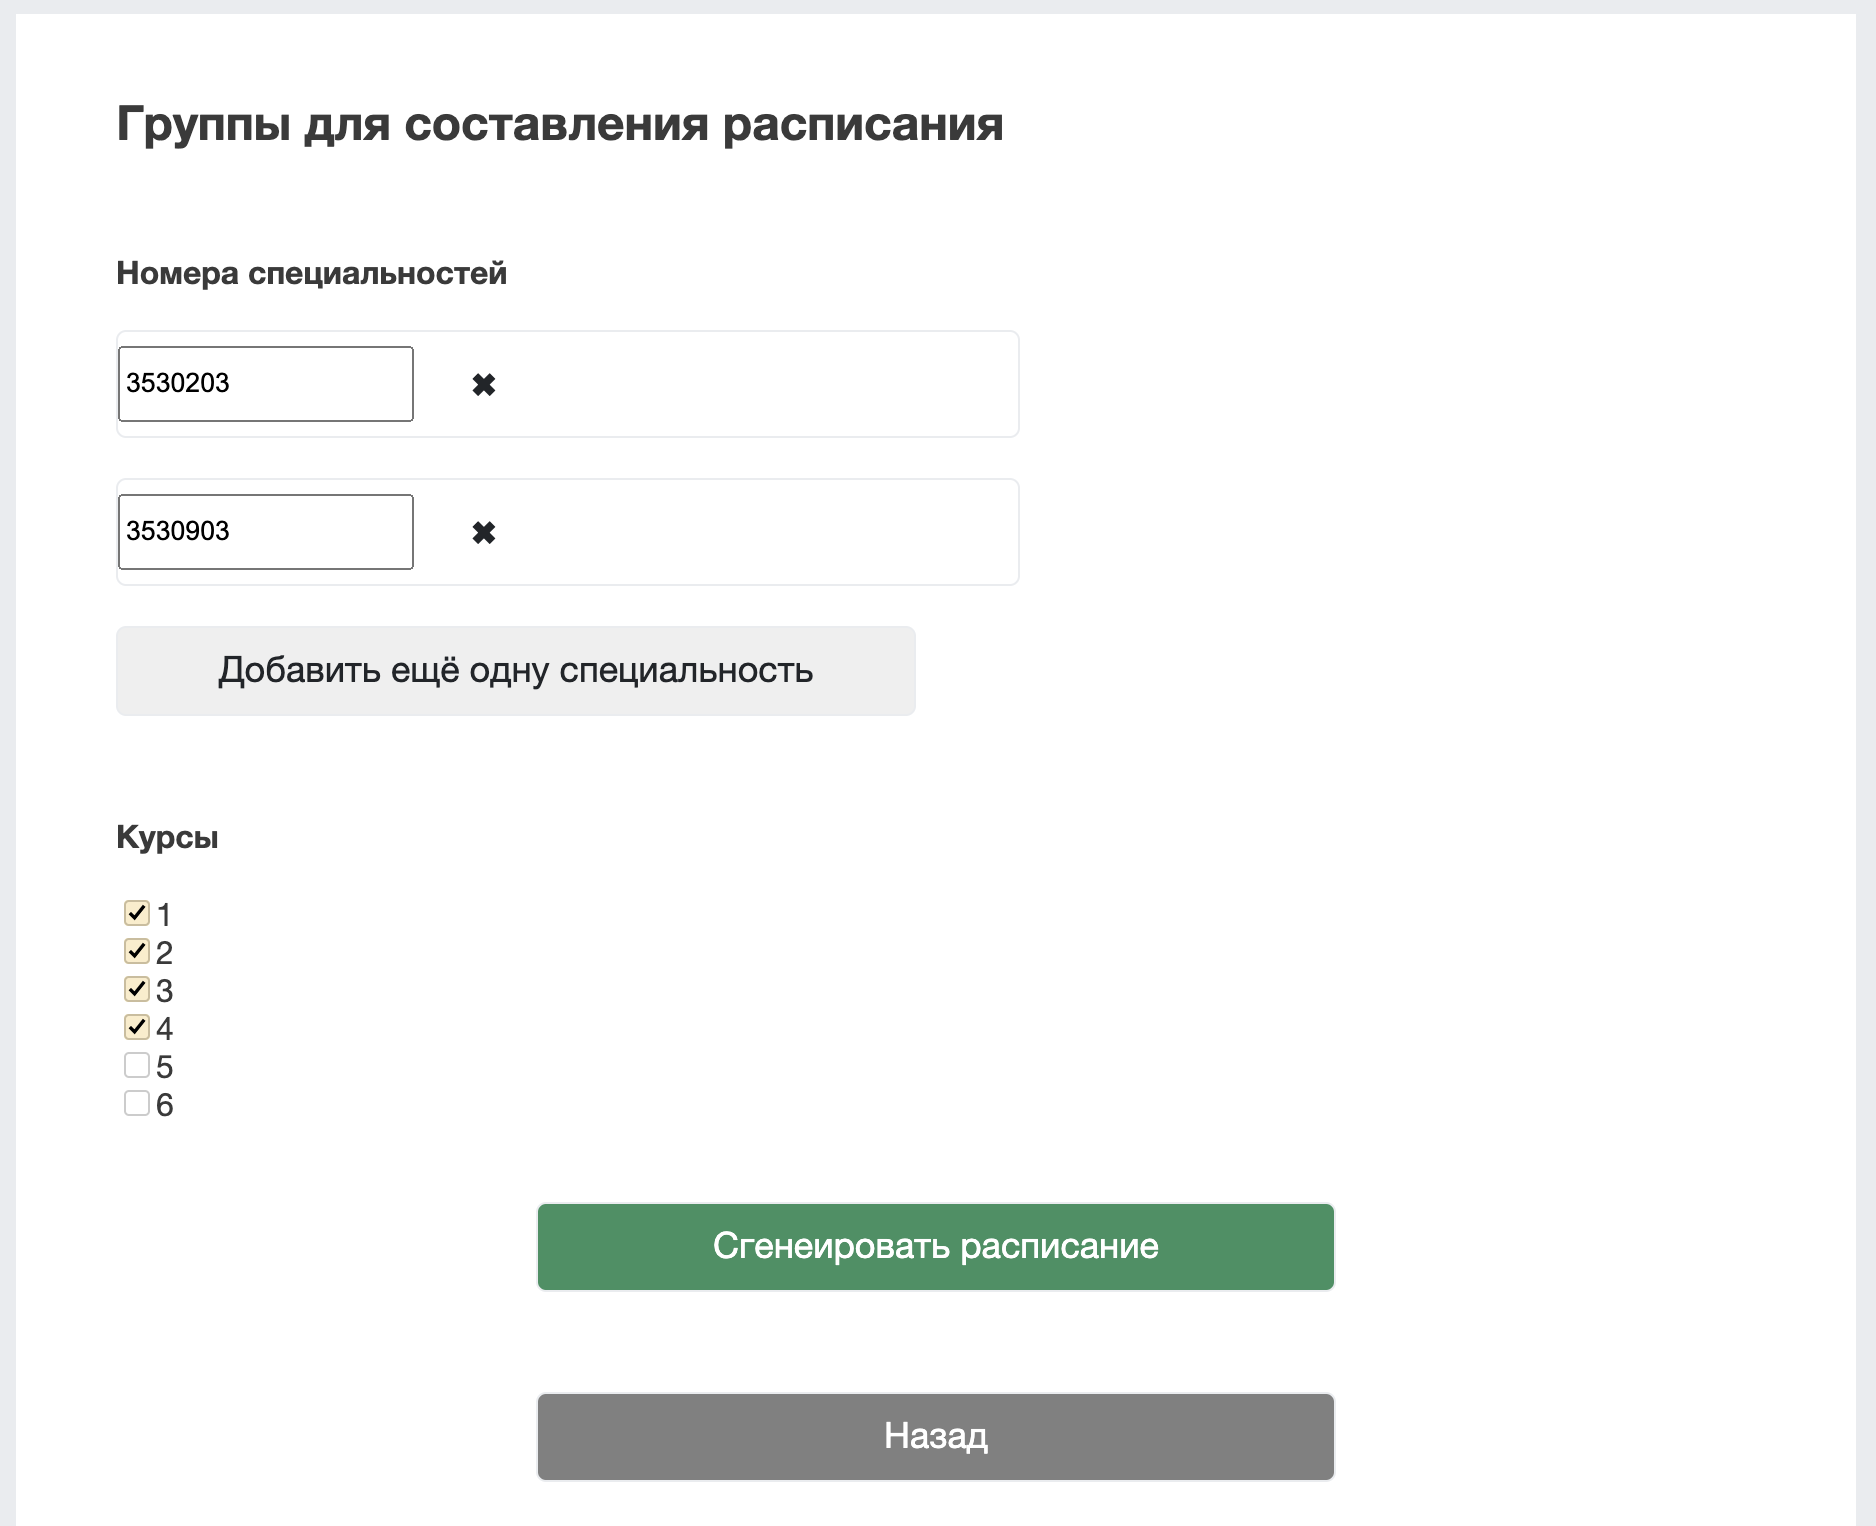
\includegraphics[ keepaspectratio=true, scale=0.4] {my_folder/images/generate}
	\captionof{figure}{Форма загрузки учебных планов}\label{fig:generate}  
	\vspace{\mfloatsep} % интервал  	
\end{minipage}
\FloatBarrier

\subsection{Spring-сервер}
Сервер имеет три основных класса-контроллера: SessionService \ref{appendix-session}, ApiRuz \ref{appendix-api} и GoogleFormService \ref{appendix-google}. Они осуществляют бизнес-логику системы и обеспечивают связь между пользователями, данными и системой. 

SessionService класс отвечает за загрузку данных о сессии от администратора. Он обрабатывает запросы, описанные в предыдущем параграфе и сохраняет данные в базе данных.

GoogleFormService класс отвечает за генерацию google-формы с предпочтениями преподавателей, загрузку данных из неё, а также из таблицы с известными аттестациями. 

Чтобы создать форму для сбора предпочтений ППС, сначала нужно выгрузить данные о преподавательских аттестациях в google-таблицу. Администратор может самостоятельно подредактировать в ней данные, например, убрав аттестации, даты и время которых определяются дирекциями других институтов. Далее администратор может создать google-форму для сбора предпочтений. Форма генерируется автоматически с помощью AppScripts скрипта \ref{appendix-appscript} по данным из таблицы.

Форма для сбора предпочтений ППС формирует для каждого преподавателя персональный опросник, в котором он определяет предпочтения только для своих аттетстаций. Фрагмент такой формы представден на рисунке \ref{fig:form2}

 \begin{minipage}{\textwidth}
	\centering
	\vspace{\mfloatsep} % интервал  	
	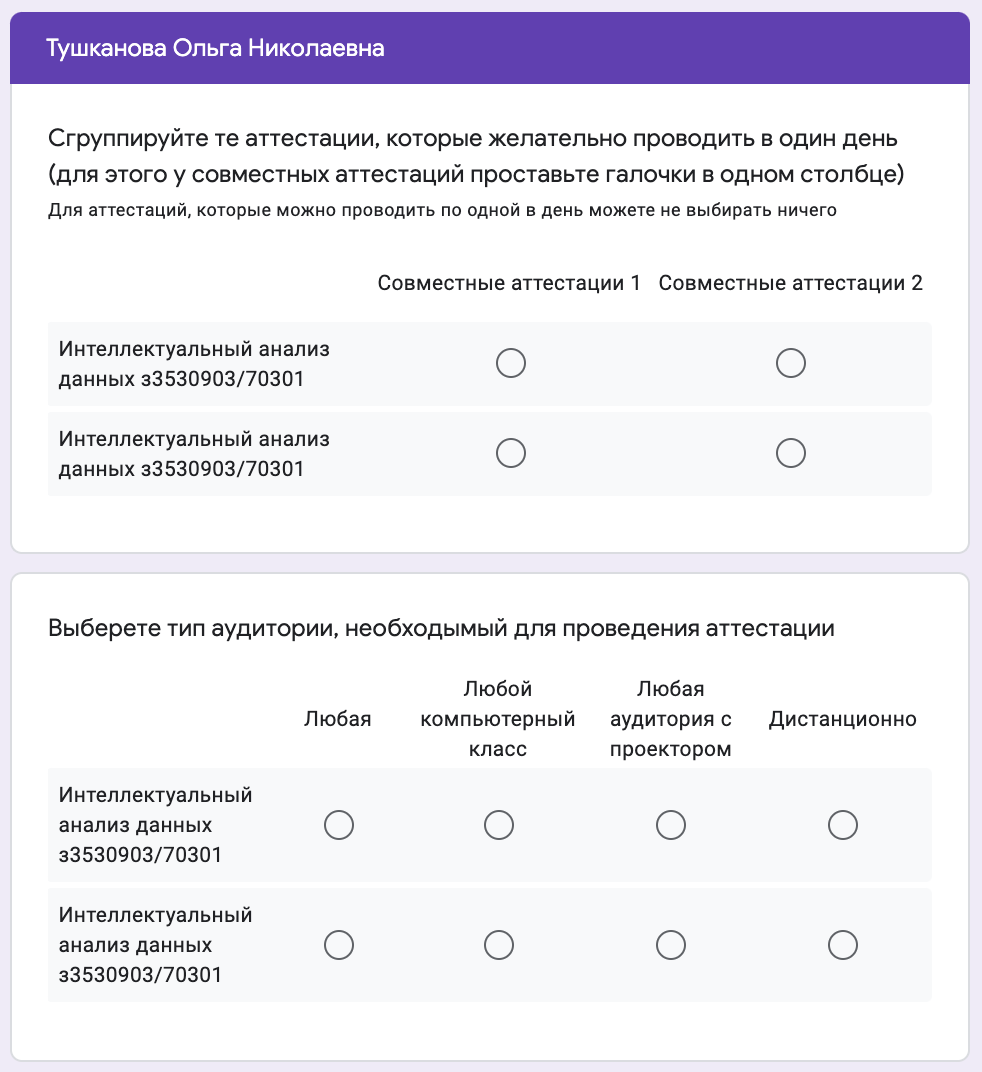
\includegraphics[ keepaspectratio=true, scale=0.6] {my_folder/images/form2}
	\captionof{figure}{Фрагмент формы для сбора предпочтений ППС}\label{fig:form2}  
	\vspace{\mfloatsep} % интервал  	
\end{minipage}

Когда предпочтения преподавателей собраны, администратор может составить расписание. Для этого сервер при помощи Google API запрашивает данные из формы и на их основе составляет предварительное расписание. Полученное расписание сервер так же записывает в таблицу.

Класс ApiRuz отвечает за получение данных с официального сайта расписания СПбПУ для формирования списка аттестаций и учёта занятости аудиторий занятиями.

Метод getDateTimesByRoomAndDate(String room, LocalDate localDate) получает даты и время, когда указанная аудитория занята.

Метод initGroups(Iterable<String> spec) получает данные о группах выбранных специальностей - их номера и курс.

Метод initRasp() для полученных раннее групп находит преподавателей, которые читают им дисциплины.

Непосредственно алгоритм генерации предварительного расписания реализован в классе ScheduleAllSolutions и подробно описан в главе \ref{ch2}.

\subsection{Хранилище данных}
Фреймворк Hibernate Spring-сервера позволяет сопоставлять java-объекты сущностям базы данных, поэтому сущности базы, перечисленные в параграфе \ref{ch1:sec1:sub3}, реализованы одноимёнными классами, помеченными аннотациями @Entity и @Data, на поля которых поставлены аннотации @Column, @ManyToOne и @OneToMany, обозначающие связи между колонками таблиц. Их код представлен в приложении \ref{appendix-classes}.

Для осуществления запросов к базе созданы классы-наследники интерфейса CrudRepository. Через них функции класса SessionDao \ref{appendix-dao}, помеченные аннотацией @Transactional, обращаются к данным.

\section{Выводы}

В результате была реализована система составления предварительного расписания сессии СПбПУ, включающая модуль веб-клиента для администратора, модуль взаимодействия с расписанием университета, модуль связи с google-таблицами для получения данных от преподавателей и модуль для генерации предварительного расписания.

Данная система может быть использована не только для составления расписания сессии, но и для  составления расписания любых событий, занимающих непрерывное время в течение одного учебного дня. Это могут быть, например, установочные занятия для студентов заочной формы обучения, экзамены дополнительной сессии, консультации по практикам или ВКР. Такое расширение применимости системы возможно благодаря аналогичному принципу генерации расписания для неповторяющися мероприятий, я формы сбора сведений о сессии и предпочтениях преподавательского состава достаточно гибкие для того, чтобы получать сведения о мероприятиях других типов.
